\ifthenelse{\equal{\Langue}{FR}}{
\chapter{Convertisseur Buck}
}{
\chapter{Buck Converter}
}

\ifthenelse{\equal{\Langue}{FR}}{
Le TP fait suite au TD sur le convertisseur Buck dont l'énoncé est rappelé ci-dessous.
L'objectif est d'utiliser le logiciel LTSpice afin de simuler le circuit et d'en comprendre le fonctionnement.
LTSpice est un logiciel fourni par Analog Device, basé sur de la simulation Spice. La documentation du logiciel est disponible sur le site d'Analog Device: \href{https://www.analog.com/en/resources/design-tools-and-calculators/ltspice-simulator/ltspice-recommended-reading-list.html}{Analog Device Website}

On souhaite alimenter un microprocesseur STM32H4 à l'aide d'une batterie. Le cahier des charges est le suivant:
}{
The lab follows the tutorial on the Buck converter, whose topic is recalled below.
The goal is to use the LTSpice software to simulate the circuit and understand its operation.
LTSpice is a software provided by Analog Device, based on Spice simulation. The software documentation is available on the Analog Device website: \href{https://www.analog.com/en/resources/design-tools-and-calculators/ltspice-simulator/ltspice-recommended-reading-list.html}{Analog Device Website}

The goal is to power a STM32H4 microprocessor using a battery. The specifications are as follows:
}

\begin{itemize}
\ifthenelse{\equal{\Langue}{FR}}{
\item Batterie LiPo 2S $V_{in} = 7.4\ V$
\item Tension d'alimentation du microprocesseur: $V_{out}=3.3\ V$
\item Ondulation de tension max en entrée du microprocesseur: $\Delta V_S = 50\ mV$
\item Courant nominal de sortie: $I_S = 200\ mA$
\item Ondulation de courant: 30\%
}{
\item LiPo 2S battery $V_{in} = 7.4\ V$
\item Microprocessor supply voltage: $V_{out}=3.3\ V$
\item Maximum voltage ripple at the microprocessor input: $\Delta V_S = 50\ mV$
\item Ratted output current: $I_S = 200\ mA$
\item Current ripple: 30\%
}
\end{itemize}

\ifthenelse{\equal{\Langue}{FR}}{
Pour cela, on souhaite utiliser le composant suivant: \textbf{LT1959} dont un extrait de la documentation 
est en annexe.
On supposera dans cet exercice que les \underline{\textbf{composants sont}} 
\underline{\textbf{parfaits}}, et que le Buck fonctionne en régime de \underline{\textbf{conduction continue}}.
}{
For this, we want to use the following component: \textbf{LT1959}, an excerpt from the documentation is in the appendix.
In this exercise, we will assume that the \underline{\textbf{components are}}
\underline{\textbf{ideal}}, and that the Buck operates in \underline{\textbf{continuous conduction mode}}.
}

\ifthenelse{\equal{\Langue}{FR}}{
\section{Préparation}
}{
\section{Preparation}
}

\begin{enumerate}
\ifthenelse{\equal{\Langue}{FR}}{
\item Tracer le circuit permettant d'utiliser ce composant en fonctionnement Buck
\item Rappeler les valeurs de (aucun calcul n'est demandé):
}{
\item Draw the circuit to use this component in Buck operation
\item Recall the values of (no calculation is required):
}
\begin{itemize}
\ifthenelse{\equal{\Langue}{FR}}{
    \item la fréquence de découpage du hacheur
    \item les valeurs de $L_1$, $C_1$ du filtrage de sortie du hacheur permettant de respecter le cahier des charges
    \item les résistances $R_1$ et $R_2$ de feedback permettant d'avoir une tension de sortie de $3.3\ V$
    \item la valeur de la résistance $R_m$ modélisant le microcontrôleur absorbant un courant nominal
    \item les valeurs de $R$ et $C$ pour l'asservissement de la tension de sortie limitant le rapport cyclique au démarrage à $\dfrac{\alpha_n}{2}$ 
    et une constante de temps du correcteur 10 fois supérieure à la constante de temps du système non corrigé
}{
    \item the switching frequency of the chopper
    \item the values of $L_1$, $C_1$ of the output filtering of the chopper to match the specifications
    \item the resistances $R_1$ and $R_2$ of feedback to have an output voltage of $3.3\ V$
    \item the value of the resistance $R_m$ modeling the microcontroller absorbing a rated current
    \item the values of $R$ and $C$ for the output voltage control limiting the duty cycle at startup to $\dfrac{\alpha_n}{2}$ 
    and a time constant of the corrector 10 times greater than the time constant of the uncorrected system
}
\end{itemize}
\end{enumerate}

\newpage
\ifthenelse{\equal{\Langue}{FR}}{
\section{Simulation du circuit}
}{
\section{Circuit Simulation}
}

\ifthenelse{\equal{\Langue}{FR}}{
Voici un bref résumé de l'interface LTSpice. Pour plus d'information, vous pouvez vous référer à la page d'Analog Device:
\href{https://www.analog.com/en/resources/design-tools-and-calculators/ltspice-simulator/ltspice-recommended-reading-list.html}{Analog Device Website}
}{
Here is a brief summary of the LTSpice interface. For more information, you can refer to the Analog Device page:
\href{https://www.analog.com/en/resources/design-tools-and-calculators/ltspice-simulator/ltspice-recommended-reading-list.html}{Analog Device Website}
}

\begin{figure}[h]
    \centering
    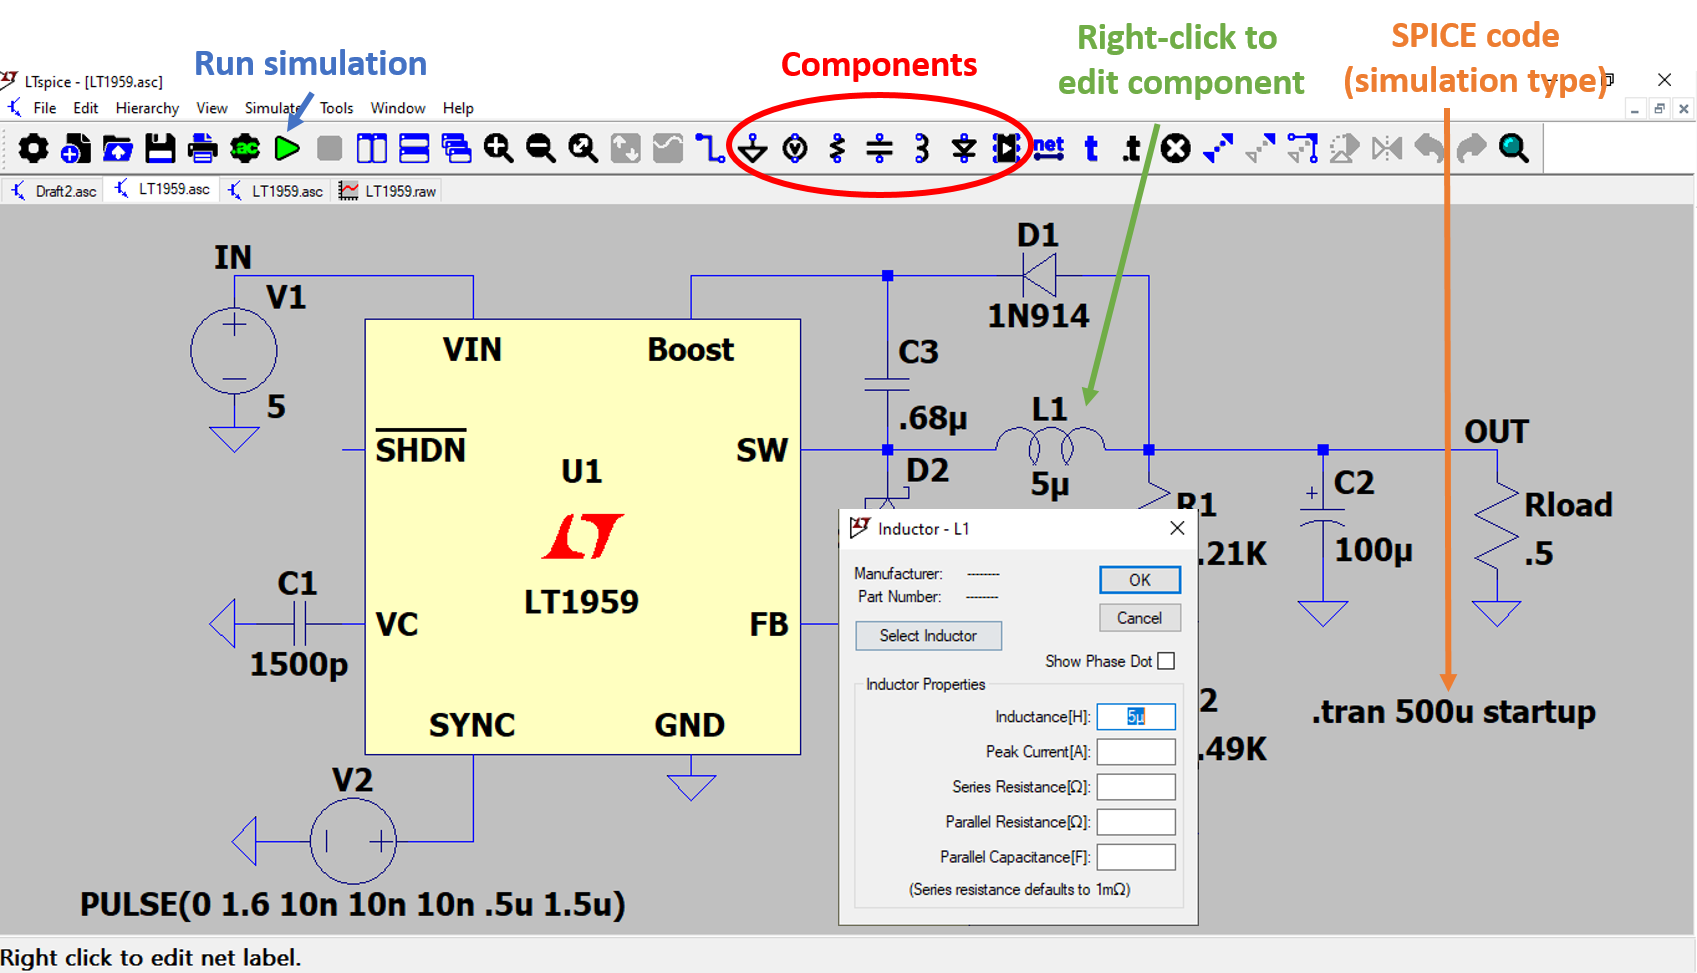
\includegraphics[width=\linewidth]{TP_Buck/fig/LTSpice.png}
\end{figure}

\begin{itemize}
\ifthenelse{\equal{\Langue}{FR}}{
\item Créer un nouveau \textit{Schematic} et placer le \textbf{LT1959}.
\item Créer le circuit de la datasheet en faisant un clic droit sur le composant $\Rightarrow$ ``\textit{Open Example Circuit}''
\item Modifier le circuit pour qu'il corresponde à la datasheet. La broche ``\textit{SYNC}'' ne sera pas utilisée.
\item Modifier les valeurs des composants afin qu'ils correspondent au cahier des charges.
\item Réaliser une simulation temporelle. Pour cela, aller dans ``\textit{Simulate}'' $\Rightarrow$ ``\textit{Configure Analysis}''
$\Rightarrow$ ``\textit{Transcient}'' et réaliser une simulation sur 3 ms.
}{
\item Create a new \textit{Schematic} and place the \textbf{LT1959}.
\item Create the circuit from the datasheet by right-clicking on the component $\Rightarrow$ ``\textit{Open Example Circuit}''
\item Modify the circuit to match the datasheet. The ``\textit{SYNC}'' pin will not be used.
\item Modify the component values to match the specifications.
\item Perform a transient simulation. To do this, go to ``\textit{Simulate}'' $\Rightarrow$ ``\textit{Configure Analysis}''
$\Rightarrow$ ``\textit{Transient}'' and perform a simulation over 3 ms.
}
\end{itemize}

\begin{enumerate}
\ifthenelse{\equal{\Langue}{FR}}{
\item Vérifier la valeur de la fréquence de découpage du convertisseur
\item Vérifier que le cahier des charges est respecté: tension de sortie, ondulation de courant, ondulation de tension
\item Le convertisseur fonctionne-t-il en régime de conduction continu ou discontinu?
}{
\item Check the value of the switching frequency of the converter
\item Check that the specifications are met: output voltage, current ripple, voltage ripple
\item Is the converter operating in continuous or discontinuous conduction mode?
}
\end{enumerate}

\newpage
\ifthenelse{\equal{\Langue}{FR}}{
\section{Influence des composants}
}{
\section{Influence of Components}
}

\begin{enumerate}
\ifthenelse{\equal{\Langue}{FR}}{
    \item Mesurer la valeur de l'ondulation de courant dans $L_1$ et de l'ondulation de tension de sortie pour différentes valeurs de $L_1$. Commenter.
    \item Mesurer la valeur de l'ondulation de tension de sortie pour différentes valeurs de $C_1$. Commenter.
    \item Déterminer la valeur de $L_1$ pour être en régime de conduction critique. Vérifier par la simulation.
}{
    \item Measure the value of the current ripple in $L_1$ and the output voltage ripple for different values of $L_1$. Comment.
    \item Measure the value of the output voltage ripple for different values of $C_1$. Comment.
    \item Determine the value of $L_1$ to be in critical conduction mode. Verify by simulation.
}
\end{enumerate}

\ifthenelse{\equal{\Langue}{FR}}{
\section{Rapidité et stabilité du système}
}{
\section{System Speed and Stability}
}

\begin{enumerate}
\ifthenelse{\equal{\Langue}{FR}}{
    \item Modifier la valeur de $C$ et mesurer le temps de réponse à 5\%. Commenter.
    \item En modifiant la valeur de $R$ déterminer la valeur maximale de la résistance à partir de laquelle le système devient instable.
    \item Ajouter un générateur de courant en parallèle de la résistance $R_s$ afin de générer un pulse de courant (une fois le système en régime permanent). 
    Ce pulse peut modéliser une perturbation CEM sur le système. Déterminer la nouvelle valeur de $R$ à partir de laquelle le système devient instable lors d'une perturbation.
}{
    \item Modify the value of $C$ and measure the 5\% time response. Comment.
    \item By modifying the value of $R$, determine the maximum value of the resistance from which the system becomes unstable.
    \item Add a current generator in parallel with the resistance $R_s$ to generate a current pulse (once the system is in steady state). 
    This pulse can model an EMC disturbance on the system. Determine the new value of $R$ from which the system becomes unstable during a disturbance.
}
\end{enumerate}